\documentclass[a4paper, 10pt]{article}
\usepackage{helvet}
\renewcommand{\familydefault}{\sfdefault}
\usepackage{pgf}
\usepackage{eurosym}
\usepackage{graphicx}
\usepackage{wasysym}
\usepackage{hyperref}
\usepackage{listings}
\usepackage{pxfonts}
\usepackage{verbatim}
\usepackage{color}
\usepackage{xcolor}
\usepackage{wrapfig}
\usepackage{enumitem}
\usepackage{booktabs}
\usepackage{gensymb}
\usepackage{tabularx}
\usepackage{currfile}

\hypersetup{
    bookmarks=true,         % show bookmarks bar?
    unicode=true,          % non-Latin characters in Acrobat’s bookmarks
    pdftoolbar=true,        % show Acrobat’s toolbar?
    pdfmenubar=true,        % show Acrobat’s menu?
    pdffitwindow=true,     % window fit to page when opened
    pdftitle={Assessments},    % title
    pdfauthor={Paul Vesey},     % author
    pdfsubject={I.C.T. Building Information Modelling},   % subject of the document
    pdfcreator={},   % creator of the document
    pdfproducer={xelatex}, % producer of the document
    pdfkeywords={'Graphics' }, % list of keywords
    pdfnewwindow=true,      % links in new PDF window
    colorlinks=true,       % false: boxed links; true: colored links
    linkcolor=violet,          % color of internal links (change box color with linkbordercolor)
    citecolor=magenta,        % color of links to bibliography
    filecolor=red,      % color of file links
    urlcolor=blue           % color of external links
}

\setlength\parindent{0pt}
\begin{document}

\lstset{language=HTML,
				basicstyle=\small,
				breaklines=true,
        numbers=left,
        numberstyle=\tiny,
        showstringspaces=false,
        aboveskip=-20pt,
        frame=leftline
        }
				
\begin{figure}
	\centering
	
\includegraphics[width=0.5\linewidth]{./Assignments/img/LITlogo}
\end{figure}


\begin{tabularx}{\textwidth}{ |l|X| }
	\hline
	\textbf{Subject:} & COMP06051-ICT \& BIM\\
	\textbf{Course:} & BEng in Civil Engineering\\
	\textbf{Session:} & Autumn 2022\\
	\textbf{Lecturer:} & Paul Vesey \footnotesize{BEng, MIE, HDip}\\
	\textbf{Filename:} & \currfilebase\\
	\hline
\end{tabularx}



\vspace{0.25cm}	
	
\begin{flushleft}
\Large\textbf{Assignment 3 (10\% of 40\%)- Microsoft Excel Regression Analysis }\\
\end{flushleft}

In this assignment you will examine and interpret construction activity data from the Central Statistic Office.  This work will involve graphing the data using an X-Y plot, complete with a trend line and regression equation.  The key deliverables for this project are:

\begin{itemize}
	\item X-Y Plot with Trace, Regression Equation and R$^{2}$ value
	\item Data Analysis Sheet (produced by Toolpak)
	\item Predictions for 2023 and 2024

\end{itemize}


\textbf{Excel Setup}

This assignment will require the Data Analysis Toolpak that ships with Microsoft Excel.  The toolpack is not enabled by default.  The toolpack is activated through the 'Options' dialogue under the File Menu in Excel as shown in Figure \ref{fig:AddinsImage}\\


\begin{figure}
	\centering
	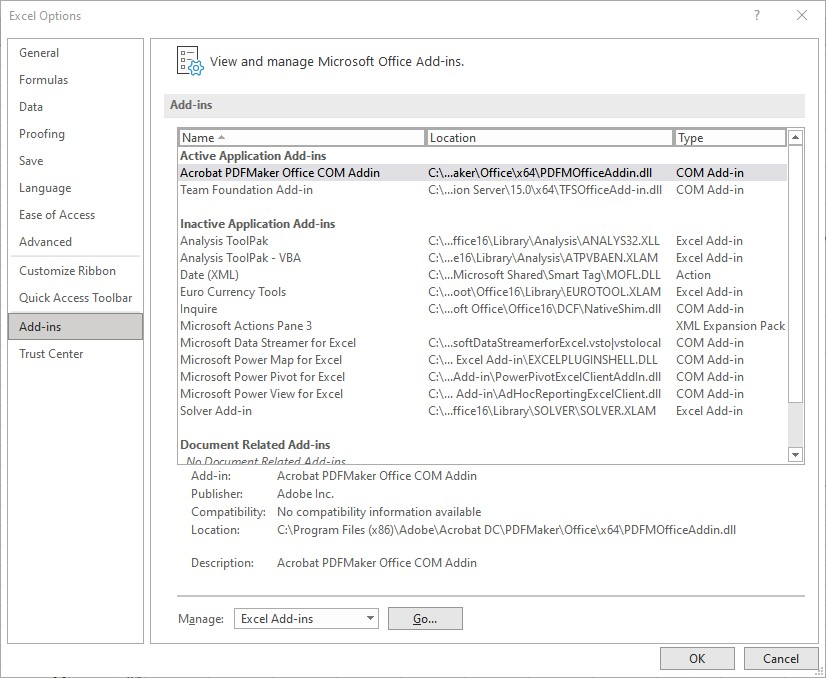
\includegraphics[width=1.0\linewidth]{./img/AddinsImage.jpg}
	\caption{Analysis Toolpak Add-ins}
	\label{fig:AddinsImage}
\end{figure}


Activate the Add-ins indicated in Figure \ref{fig:AddInSelection}.\\

\begin{figure}
	\centering
	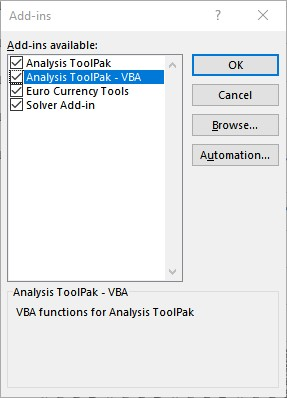
\includegraphics[width=0.6\linewidth]{./img/AddInSelection.jpg}
	\caption{Data Analysis Tool Selection}
	\label{fig:AddInSelection}
\end{figure}


Once the Add-ins have been successfully activated a new tool panel will be available under the 'Data' tool ribbon.  An image of the tool is shown in Figure \ref{fig:DataAnalysisTools}\\

\begin{figure}
	\centering
	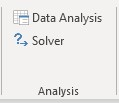
\includegraphics[width=0.25\linewidth]{./img/DataAnalysisTools.jpg}
	\caption{Data Analysis Toolbox on Excel Ribbon}
	\label{fig:DataAnalysisTools}
\end{figure}

\newpage

\textbf{Data Analysis}

An Excel file containing the data for analysis has been provided to you.  The goal is to create an X-Y plot of the 'Production Index in Building and Construction', produce trend line, complete with Regression Equation and R$^{2}$ value.  This will produce results as shown in Figure \ref{fig:Excel1}.\\


\begin{figure}
	\centering
	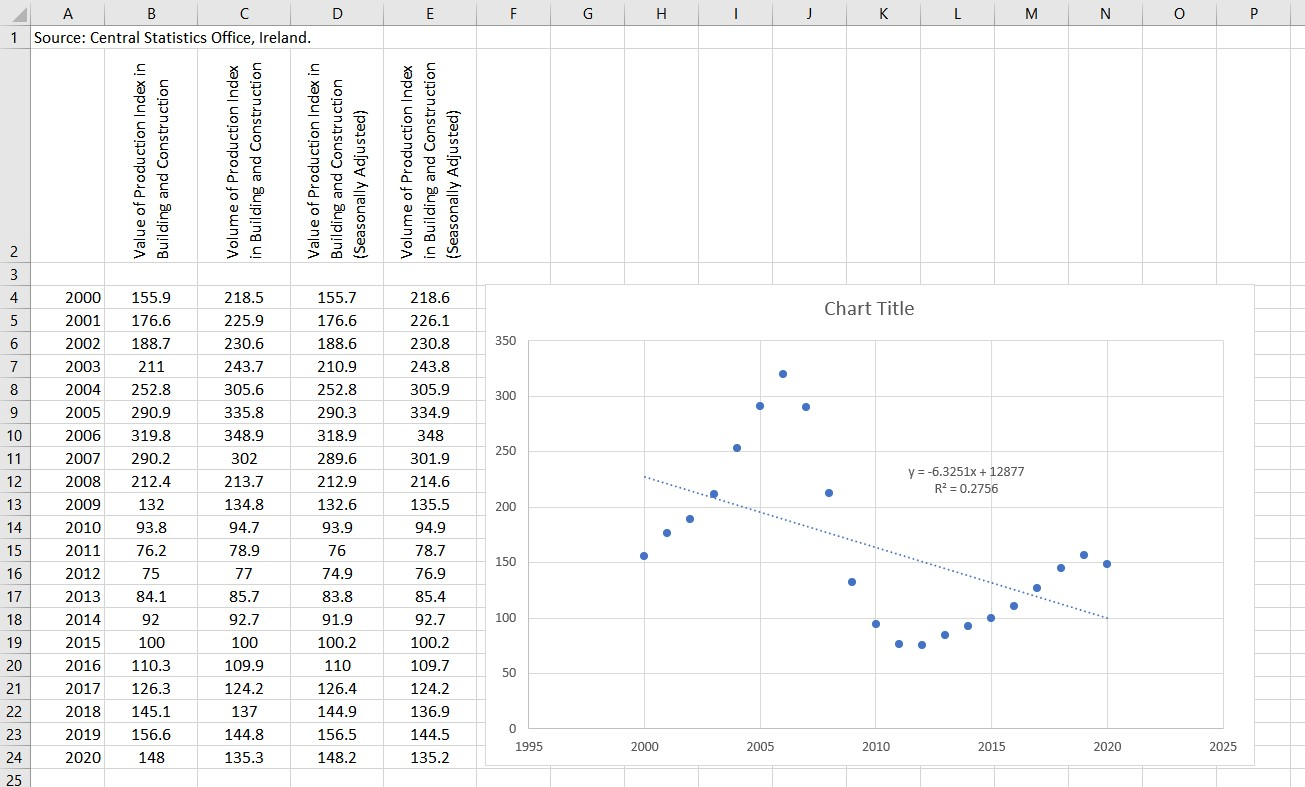
\includegraphics[width=1.0\linewidth]{./img/Excel1.jpg}
	\caption{First Stage of Analysis}
	\label{fig:Excel1}
\end{figure}

You will see from the image in Figure \ref{fig:Excel1} that the R$^{2}$ value is very low, indicating that the regression line is a poor fit to the data.  The goal of this assignment is to produce a regression line and equation with an R$^{2}$ value of 0.90 or better.  In order to achieve this you will need to select the most appropriate data to predict Construction Output for the years 2023 and 2024.\\

\begin{figure}
	\centering
	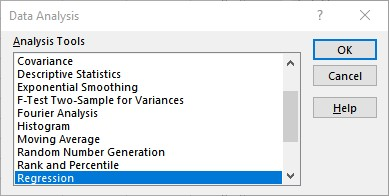
\includegraphics[width=0.8\linewidth]{./img/DataAnalysisWindow.jpg}
	\caption{Data Analysis - Regression Tool}
	\label{fig:DataAnalysisWindow}
\end{figure}


\begin{figure}
	\centering
	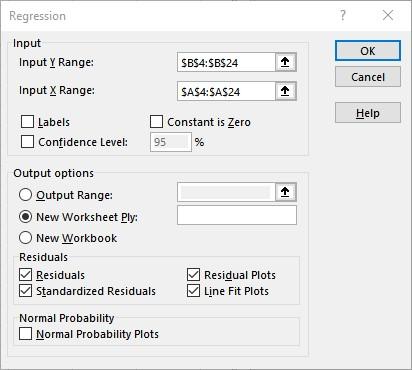
\includegraphics[width=0.8\linewidth]{./img/AnalysisSettings.jpg}
	\caption{Regression Dialog Box}
	\label{fig:AnalysisSettings}
\end{figure}


A more complete analysis is possible using the Data Analysis tools activated previously. Selecting the Data Analysis tool under the Data ribbon will open the dialogue box shown in Figure \ref{fig:DataAnalysisWindow}.  Selecting the 'Regression' tool will activate the Analysis Settings Dialogue shown in Figure \ref{fig:AnalysisSettings} \\

The regression tool will produce the analysis shown in Figure \ref{fig:Excel2}.  


\begin{figure}
	\centering
	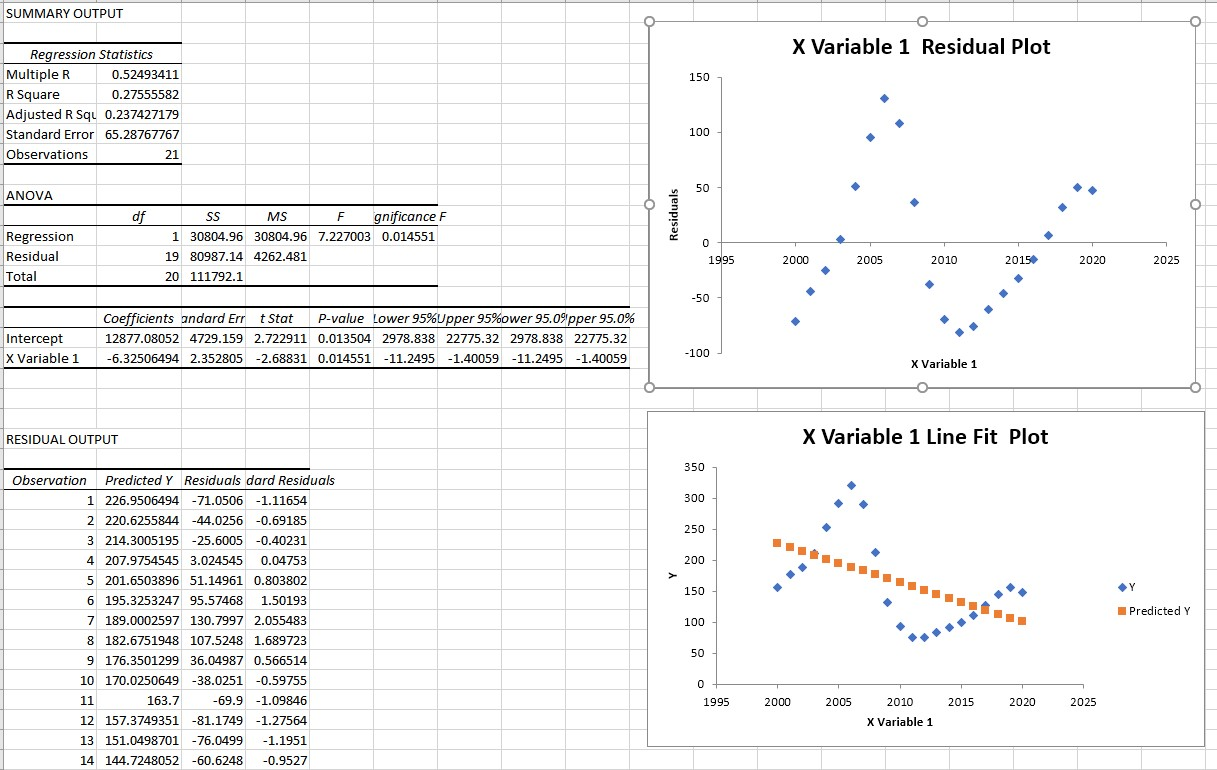
\includegraphics[width=1.0\linewidth]{./img/Excel2.jpg}
	\caption{Regression Analysis from Toolkit}
	\label{fig:Excel2}
\end{figure}

The final part of the assignment is to use your regression equation to produce projections for Years 2023 and 2034.  Your equation will be in the form:

\begin{center}
	$y = mx +c $
\end{center}

where $y$ is your index value, $x$ is the input year, and $m$ and $c$ are your regression coefficients.



\newpage


\textbf{Submission}\\
Your completed assignment comprising of a single Excel file is to be uploaded to MS Teams on or before the date and time indicated.  

\vspace{0.5cm}

\textbf{Late Submission}\\
Failure to submit your assignment on or before the date and time indicated on Teams will result in a penalty of 5\% per day or part thereof.

\vspace{0.5cm}
\textbf{Marking Scheme}

\begin{table}[h!]
     \begin{center}
     \begin{tabular}{p{9cm}  p{2cm} }
     \toprule
      \textbf\large{Element} & \textbf\large{Proportion} \\ 
    \cmidrule(r){1-1}\cmidrule(lr){2-2}
    	Setup Excel for Data Analysis 		 	& 20\%\\
    	X-Y Plot with Trace, Regression Equation and R$^{2}$ value	& 30\%\\
        Data Analysis Sheet (produced by Toolpak)  	& 20\%\\
        Predictions for 2023 and 2024   	& 30\%\\
      \bottomrule
      \end{tabular}
      \label{tbl:markSchemeAsmt3}
      \end{center}
 \end{table}

\end{document}